% Generated by analyze_t1b.js - paste before \end{document}
\subsection{T1-b -- Effect of the block-cutting timeout}
The T1 procedure was repeated after changing only the channel parameter \texttt{BatchTimeout} through a signed
channel configuration update (all other parameters unchanged): 1\,s (5 runs $\times$ 30
iterations, 16:25--16:42 CEST) and 0.5\,s (5 runs $\times$
30 iterations, 16:42--16:51 CEST), each with 2 excluded warm-up
iterations. The 2\,s values are those of T1. All 3300 additional requests completed successfully
(0 failures). The original value of 2\,s was restored at the end of the experiment.

\begin{table}[H]
\centering\small
\caption{T1-b: mean latency (ms) of each operation for \texttt{BatchTimeout} = 2\,s, 1\,s and 0.5\,s.
End-to-end latency and endorsement phase (chaincode execution) of state-changing operations; end-to-end latency
of read-only queries.}
\label{tab:t1b}
\setlength{\tabcolsep}{4pt}
\begin{tabular}{lrrrrrr}
\toprule
 & \multicolumn{3}{c}{End-to-end} & \multicolumn{3}{c}{Endorse} \\
\cmidrule(lr){2-4}\cmidrule(lr){5-7}
Operation & 2\,s & 1\,s & 0.5\,s & 2\,s & 1\,s & 0.5\,s \\
\midrule
\multicolumn{7}{l}{\emph{State-changing}} \\
Production registration & 2044.6 & 1040.3 & 531.2 & 13.2 & 12.6 & 7.9 \\
Transformation (mass balance) & 2050.4 & 1044.1 & 534.6 & 17.9 & 16.2 & 11.1 \\
Package creation & 2045.0 & 1041.1 & 532.4 & 14.1 & 13.0 & 8.9 \\
Binding registration (PDC) & 2059.6 & 1052.7 & 542.4 & 25.5 & 22.9 & 18.1 \\
Certificate consumption & 2043.0 & 1038.0 & 532.5 & 12.0 & 10.6 & 8.5 \\
Repeated scan (consumed cert.) & 2047.8 & 1042.0 & 532.1 & 16.3 & 14.3 & 9.9 \\
\midrule
\multicolumn{7}{l}{\emph{Read-only}} \\
Production query & 6.7 & 6.2 & 4.2 & \multicolumn{3}{c}{--} \\
Certificate query & 6.4 & 5.6 & 4.3 & \multicolumn{3}{c}{--} \\
Certificate integrity check & 5.4 & 4.8 & 3.7 & \multicolumn{3}{c}{--} \\
Authorization check & 4.9 & 4.4 & 3.4 & \multicolumn{3}{c}{--} \\
UID verification (PDC) & 10.2 & 8.9 & 7.1 & \multicolumn{3}{c}{--} \\
\bottomrule
\end{tabular}
\end{table}

\begin{figure}[H]
\centering
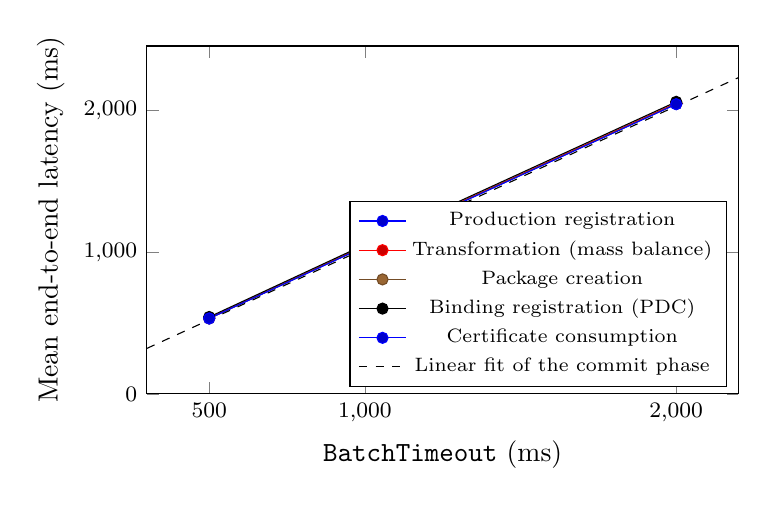
\begin{tikzpicture}
\begin{axis}[width=0.75\linewidth, height=6cm, xlabel={\texttt{BatchTimeout} (ms)},
  ylabel={Mean end-to-end latency (ms)}, xtick={500,1000,2000}, xmin=300, xmax=2200, ymin=0,
  legend style={font=\scriptsize, at={(0.98,0.02)}, anchor=south east}, tick label style={font=\footnotesize}]
\addplot+[mark=*] coordinates {(2000,2044.6) (1000,1040.3) (500,531.2)};
\addlegendentry{Production registration}
\addplot+[mark=*] coordinates {(2000,2050.4) (1000,1044.1) (500,534.6)};
\addlegendentry{Transformation (mass balance)}
\addplot+[mark=*] coordinates {(2000,2045.0) (1000,1041.1) (500,532.4)};
\addlegendentry{Package creation}
\addplot+[mark=*] coordinates {(2000,2059.6) (1000,1052.7) (500,542.4)};
\addlegendentry{Binding registration (PDC)}
\addplot+[mark=*] coordinates {(2000,2043.0) (1000,1038.0) (500,532.5)};
\addlegendentry{Certificate consumption}
\addplot[dashed, domain=300:2200] {19.3 + 1.0051*x};
\addlegendentry{Linear fit of the commit phase}
\end{axis}
\end{tikzpicture}
\caption{T1-b: end-to-end latency of state-changing operations as a function of \texttt{BatchTimeout}.}
\label{fig:t1b}
\end{figure}

\paragraph{Observations.}
\begin{itemize}
  \item \textbf{Causal confirmation.} The mean commit-phase latency of state-changing operations follows
        $L^{\mathrm{com}} \approx 19.3\,\mathrm{ms} + 1.005 \cdot \texttt{BatchTimeout}$
        ($R^2 = 1.0000$): reducing the timeout from 2\,s to 0.5\,s reduces the end-to-end latency of
        every write by the same amount, which confirms that under sequential submission the write latency is
        determined by the block-cutting configuration of the ordering service.
  \item \textbf{Chaincode cost is unaffected.} The endorsement phase remains in the same range
        (12.0--25.5\,ms at 2\,s, 7.9--18.1\,ms at 0.5\,s), as do read-only queries
        (4.9--10.2\,ms and 3.4--7.1\,ms): the cost of the Enhanced SPECTRA mechanisms is
        independent of the ordering configuration.
  \item \textbf{Deployment implication.} \texttt{BatchTimeout} is a deployment trade-off: a shorter timeout lowers
        the latency of individual transactions under light load, at the cost of smaller blocks and higher
        per-transaction block overhead. Throughput under load is evaluated in T2 with the default value of 2\,s.
\end{itemize}
